% ****************************************************************************************
% ************************     REPORTE DE BASES DE DATOS    ******************************
% ****************************************************************************************


% =======================================================
% =======         HEADER FOR DOCUMENT        ============
% =======================================================
    % *********   DOCUMENT ITSELF   **************
    \documentclass[12pt, fleqn]{report}                             %Type of docuemtn and size of font and left eq
    \usepackage[margin=1.2in]{geometry}                             %Margins and Geometry pacakge
    \usepackage{ifthen}                                             %Allow simple programming
    \usepackage{hyperref}                                           %Create MetaData for a PDF and LINKS!
    \usepackage{pdfpages}                                           %Create MetaData for a PDF and LINKS!
    \hypersetup{pageanchor=false}                                   %Solve 'double page 1' warnings in build
    \setlength{\parindent}{0pt}                                     %Eliminate ugly indentation
    \author{Oscar Andrés Rosas}                                     %Who I am

    % *********   LANGUAJE AND UFT-8   *********
    \usepackage[spanish]{babel}                                     %Please use spanish
    \usepackage[utf8]{inputenc}                                     %Please use spanish - UFT
    \usepackage[T1]{fontenc}                                        %Please use spanish
    \usepackage{textcmds}                                           %Allow us to use quoutes
    \usepackage{changepage}                                         %Allow us to use identate paragraphs

    % *********   MATH AND HIS STYLE  *********
    \usepackage{ntheorem, amsmath, amssymb, amsfonts}               %All fucking math, I want all!
    \usepackage{mathrsfs, mathtools, empheq}                        %All fucking math, I want all!
    \usepackage{centernot}                                          %Allow me to negate a symbol
    \decimalpoint                                                   %Use decimal point

    % *********   GRAPHICS AND IMAGES *********
    \usepackage{graphicx}                                           %Allow to create graphics
    \usepackage{wrapfig}                                            %Allow to create images
    \graphicspath{ {Graphics/} }                                    %Where are the images :D

    % *********   LISTS AND TABLES ***********
    \usepackage{listings}                                           %We will be using code here
    \usepackage[inline]{enumitem}                                   %We will need to enumarate
    \usepackage{tasks}                                              %Horizontal lists
    \usepackage{longtable}                                          %Lets make tables awesome
    \usepackage{booktabs}                                           %Lets make tables awesome
    \usepackage{tabularx}                                           %Lets make tables awesome
    \usepackage{multirow}                                           %Lets make tables awesome
    \usepackage{multicol}                                           %Create multicolumns

    % *********   HEADERS AND FOOTERS ********
    \usepackage{fancyhdr}                                           %Lets make awesome headers/footers
    \pagestyle{fancy}                                               %Lets make awesome headers/footers
    \setlength{\headheight}{16pt}                                   %Top line
    \setlength{\parskip}{0.5em}                                     %Top line
    \renewcommand{\footrulewidth}{0.5pt}                            %Bottom line

    \lhead{                                                         %Left Header
        \hyperlink{chapter.\arabic{chapter}}                        %Make a link to the current chapter
        {\normalsize{\textsc{\nouppercase{\leftmark}}}}             %And fot it put the name
    }

    \rhead{                                                         %Right Header
        \hyperlink{section.\arabic{chapter}.\arabic{section}}       %Make a link to the current chapter
            {\footnotesize{\textsc{\nouppercase{\rightmark}}}}      %And fot it put the name
    }

    \rfoot{\textsc{\small{\hyperref[sec:Index]{Ve al Índice}}}}     %This will always be a footer  

    \fancyfoot[L]{                                                  %Algoritm for a changing footer
        \footnotesize{\textsc{Maneja tu Cine - Bases de Datos}}      %Titulo
    }
    
       
    
% ========================================
% ===========   COMMANDS    ==============
% ========================================

    % =====  GENERAL TEXT  ==========
    \newcommand \Quote {\qq}                                        %Use: \Quote to use quotes
    \newcommand \Over {\overline}                                   %Use: \Bar to use just for short
    \newcommand \ForceNewLine {$\Space$\\}                          %Use it in theorems for example
    
    \newenvironment{Indentation}[1][0.75em]                         %Use: \begin{Inde...}[Num]...\end{Inde...}
    {\begin{adjustwidth}{#1}{}}                                     %If you dont put nothing i will use 0.75 em
    {\end{adjustwidth}}                                             %This indentate a paragraph
    \newenvironment{SmallIndentation}[1][0.75em]                    %Use: The same that we upper one, just 
    {\begin{adjustwidth}{#1}{}\begin{footnotesize}}                 %footnotesize size of letter by default
    {\end{footnotesize}\end{adjustwidth}}                           %that's it


    % =====  GENERAL MATH  ==========
    \DeclareMathOperator \Space {\quad}                             %Use: \Space for a cool mega space
    \DeclareMathOperator \MiniSpace {\;}                            %Use: \Space for a cool mini space
    \newcommand \Such {\MiniSpace|\MiniSpace}                       %Use: \Such like in sets
    \newcommand \Also {\MiniSpace \text{y} \MiniSpace}              %Use: \Also so it's look cool
    \newcommand \Remember[1]{\Space\text{\scriptsize{#1}}}          %Use: \Remember so it's look cool

    \newtheorem{Theorem}{Teorema}[section]                          %Use: \begin{Theorem}[Name]\label{Nombre}...
    \newtheorem{Corollary}{Colorario}[Theorem]                      %Use: \begin{Corollary}[Name]\label{Nombre}...
    \newtheorem{Lemma}[Theorem]{Lemma}                              %Use: \begin{Lemma}[Name]\label{Nombre}...
    \newtheorem{Definition}{Definición}[section]                    %Use: \begin{Definition}[Name]\label{Nombre}...

    \newcommand{\Set}[1]{\left\{ \MiniSpace #1 \MiniSpace \right\}} %Use: \Set {Info}
    \newcommand{\Brackets}[1]{\left[ #1 \right]}                    %Use: \Brackets {Info} 
    \newcommand{\Wrap}[1]{\left( #1 \right)}                        %Use: \Wrap {Info} 
    \newcommand{\pfrac}[2]{\Wrap{\dfrac{#1}{#2}}}                   %Use: Put fractions in parentesis

    \newenvironment{MultiLineEquation}[1]                           %Use: To create MultiLine equations
        {\begin{equation}\begin{alignedat}{#1}}                     %Use: \begin{Multi..}{Num. de Columnas}
        {\end{alignedat}\end{equation}}                             %And.. that's it!
    \newenvironment{MultiLineEquation*}[1]                          %Use: To create MultiLine equations
        {\begin{equation*}\begin{alignedat}{#1}}                    %Use: \begin{Multi..}{Num. de Columnas}
        {\end{alignedat}\end{equation*}}                            %And.. that's it!


    % =====  LOGIC  ==================
    \DeclareMathOperator \doublearrow {\leftrightarrow}             %Use: \doublearrow for a double arrow
    \newcommand \lequal {\MiniSpace \Leftrightarrow \MiniSpace}     %Use: \lequal for a double arrow
    \newcommand \linfire {\MiniSpace \Rightarrow \MiniSpace}        %Use: \lequal for a double arrow
    \newcommand \longto {\longrightarrow}                           %Use: \longto for a long arrow

    % =====  NUMBER THEORY  ==========
    \DeclareMathOperator \Naturals  {\mathbb{N}}                     %Use: \Naturals por Notation
    \DeclareMathOperator \Primes    {\mathbb{P}}                     %Use: \Naturals por Notation
    \DeclareMathOperator \Integers  {\mathbb{Z}}                     %Use: \Integers por Notation
    \DeclareMathOperator \Racionals {\mathbb{Q}}                     %Use: \Racionals por Notation
    \DeclareMathOperator \Reals     {\mathbb{R}}                     %Use: \Reals por Notation
    \DeclareMathOperator \Complexs  {\mathbb{C}}                     %Use: \Complex por Notation

    % === LINEAL ALGEBRA & VECTORS ===
    \DeclareMathOperator \LinealTransformation {\mathcal{T}}        %Use: \LinealTransformation for a cool T
    \newcommand{\Mag}[1]{\left| #1 \right|}                         %Use: \Mag {Info} 

    \newcommand{\pVector}[1]{                                       %Use: \pVector {Matrix Notation} use parentesis
        \ensuremath{\begin{pmatrix}#1\end{pmatrix}}                 %Example: \pVector{a\\b\\c} or \pVector{a&b&c} 
    }
    \newcommand{\lVector}[1]{                                       %Use: \lVector {Matrix Notation} use a abs 
        \ensuremath{\begin{vmatrix}#1\end{vmatrix}}                 %Example: \lVector{a\\b\\c} or \lVector{a&b&c} 
    }
    \newcommand{\bVector}[1]{                                       %Use: \bVector {Matrix Notation} use a brackets 
        \ensuremath{\begin{bmatrix}#1\end{bmatrix}}                 %Example: \bVector{a\\b\\c} or \bVector{a&b&c} 
    }
    \newcommand{\Vector}[1]{                                        %Use: \Vector {Matrix Notation} no parentesis
        \ensuremath{\begin{matrix}#1\end{matrix}}                   %Example: \Vector{a\\b\\c} or \Vector{a&b&c}
    }

    % MATRIX
    \makeatletter                                                   %Example: \begin{matrix}[cc|c]
    \renewcommand*\env@matrix[1][*\c@MaxMatrixCols c] {             %WTF! IS THIS
        \hskip -\arraycolsep                                        %WTF! IS THIS
        \let\@ifnextchar\new@ifnextchar                             %WTF! IS THIS
        \array{#1}                                                  %WTF! IS THIS
    }                                                               %WTF! IS THIS
    \makeatother                                                    %WTF! IS THIS

    % TRIGONOMETRIC FUNCTIONS
    \newcommand{\Cos}[1]{\cos\Wrap{#1}}                             %Simple wrappers
    \newcommand{\Sin}[1]{\sin\Wrap{#1}}                             %Simple wrappers

    % === COMPLEX ANALYSIS ===
    \newcommand \Cis[1]  {\Cos{#1} + i \Sin{#1}}                    %Use: \Cis for cos(x) + i sin(x)
    \newcommand \pCis[1] {\Wrap{\Cis{#1}}}                          %Use: \pCis for the same ut parantesis
    \newcommand \bCis[1] {\Brackets{\Cis{#1}}}                      %Use: \bCis for the same to Brackets

    % === CALCULUS ===
    \newcommand \MiniDerivate[1][x] {\dfrac{d}{d #1}}               %Use: \MiniDerivate for simple use
    \newcommand \Derivate[2]                                        %Complete Derivate -- [f(x)][x]
        {\dfrac{d \; #1}{d #2}}                                     %Use: \Partial for simple use
    
    \newcommand \MiniUpperDerivate[2]                               %Mini Derivate High Orden Derivate -- [x][1]
        {\dfrac{d^{#2}}{d#1^{#2}}}                                  %Mini Derivate High Orden Derivate
    \newcommand \UpperDerivate[3]                                   %Complete High Orden Derivate -- [f(x)][x][1]
        {\dfrac{d^{#3} \; #1}{d#2^{#3}}}                            %Use: \UpperDerivate for simple use
    
    \newcommand \MiniPartial[1][x] {\dfrac{\partial}{\partial #1}} %Use: \MiniDerivate for simple use
    \newcommand \Partial[2]                                        %Complete Derivate -- [f(x)][x]
        {\dfrac{\partial \; #1}{\partial #2}}                      %Use: \Partial for simple use
    
    \newcommand \MiniUpperPartial[2]                                %Mini Derivate High Orden Derivate -- [x][1] 
        {\dfrac{\partial^{#2}}{\partial #1^{#2}}}                   %Mini Derivate High Orden Derivate
    \newcommand \UpperPartial[3]                                    %Complete High Orden Derivate -- [f(x)][x][1]
        {\dfrac{\partial^{#3} \; #1}{\partial#2^{#3}}}              %Use: \UpperDerivate for simple use


    % =====  GENERAL COLOR  =========
    \definecolor{IndigoMD}{HTML}{3F51B5}                            %Use: Color :D
    \definecolor{DeepPurpleMD}{HTML}{673AB7}                        %Use: Color :D
    \definecolor{TealMD}{HTML}{009688}                              %Use: Color :D        
    \definecolor{BlueGrey800MD}{HTML}{37474F}                       %Use: Color :D
    \definecolor{BlueGrey100MD}{HTML}{CFD8DC}                       %Use: Color :D
    \definecolor{IndigoMD}{HTML}{3F51B5}                            %Use: Color :D
    \definecolor{Green100MD}{HTML}{DCEDC8}                          %Use: Color :D

    \newenvironment{ColorText}[1]{                                  %Use: \begin{ColorText}
        \leavevmode\color{#1}\ignorespaces}                         %That's is!


    % =====  CODE EDITOR =========
    \lstdefinestyle{CompilandoStyle} {                              %This is Code Style
        backgroundcolor=\color{BlueGrey800MD},                      %Background Color  
        basicstyle=\color{white}\fontsize{9}{11}\ttfamily,          %Estilo
        commentstyle=\color{BlueGrey100MD},                         %Comment color
        stringstyle=\color{TealMD},                                 %String color
        keywordstyle=\color{Green100MD},                            %keywords color
        numberstyle=\tiny\color{TealMD},                            %Size of a number
        frame=shadowbox,                                            %Adds a frame around the code
        breakatwhitespace=true,                                     %Style                       
        breaklines=true,                                            %Style                   
        keepspaces=true,                                            %Style                   
        numbers=left,                                               %Style                   
        numbersep=10pt,                                             %Style 
        xleftmargin=\parindent,                                     %Style 
        tabsize=4                                                   %Style 
    }
 
    \lstset{style=CompilandoStyle}                                  %Use this style


  

% =====================================================
% ============        COVER PAGE       ================
% =====================================================
\begin{document}
\begin{titlepage}

    \center
    % ============ UNIVERSITY NAME AND DATA =========
    \textsc{\Large Bases de Datos}\\[0.5cm] 
    \textsc{\large 2CM12}\\[1.5cm]

    % ============ NAME OF THE DOCUMENT  ============
    \rule{\linewidth}{0.5mm} \\[1.0cm]
        { \huge \bfseries Manage Your Cinema}\\[1.0cm] 
    \rule{\linewidth}{0.5mm} \\[2.0cm]
     
    % ============  MY INFORMATION  =================
    \begin{minipage}{0.4\textwidth}
        \begin{flushleft} \large
            \textbf{\textsc{Alumnos:}}\\
            \small{
                Maya Rocha Luis Emmanuel        \\
                Rosas Hernández Óscar Andrés    \\
                Dominguez Lopez Humberto        \\
                Hernández Ruiz Rafael
            }
        \end{flushleft}
    \end{minipage}
    ~
    \begin{minipage}{0.4\textwidth}
        \begin{flushright} \large
            \textbf{\textsc{Profesor: }}\\
            Euler Hernández Contreras
        \end{flushright}
    \end{minipage}\\[3,5cm]

    % ====== SEMI TITLE ==========
    {\LARGE Reporte de Bases de Datos}
    \vfill

\end{titlepage}




% =====================================================
% ========                INDICE              =========
% =====================================================
\tableofcontents{}
\label{sec:Index}

\clearpage


% ======================================================================================
% ===============================   PRIMERA PARTE     ==================================
% ======================================================================================
\chapter{Primer Parte}
\clearpage

    % ===============================================================
    % =====================     INTRODUCCION   ======================
    % ===============================================================
    \section{Introducción}

        Como proyecto final de Bases de Datos nos disponemos a crear un Sistema basado en Web 
        (usando sobretodo PHP y el framework MaterializeCSS) para poder gestionar un Cine:
        \begin{itemize}
            \item Películas
            \item Horarios
            \item Dulceria
            \item Empleados
            \item Organización en general
        \end{itemize}


        Toda la información del sistema será almacenada en una base de datos creada con MySQL
        y que se comunicará con nuestra aplicación web usando las funciones de PHP con MySQL.

        \clearpage

        \begin{figure}[h!]
            \centering
            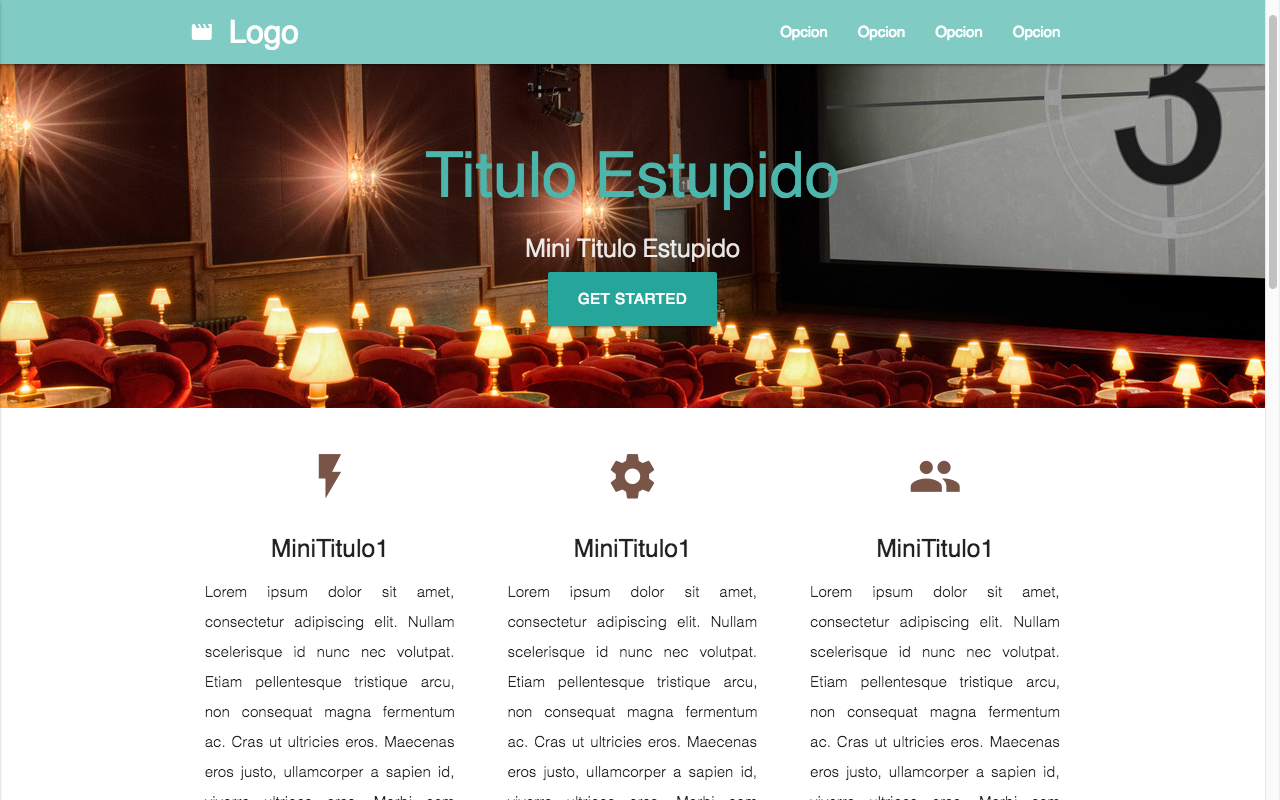
\includegraphics[width=0.80\textwidth]{Examples0.png}
            \caption{Boceto de FrontEnd de la aplicación web}
        \end{figure}

        \begin{figure}[h!]
            \centering
            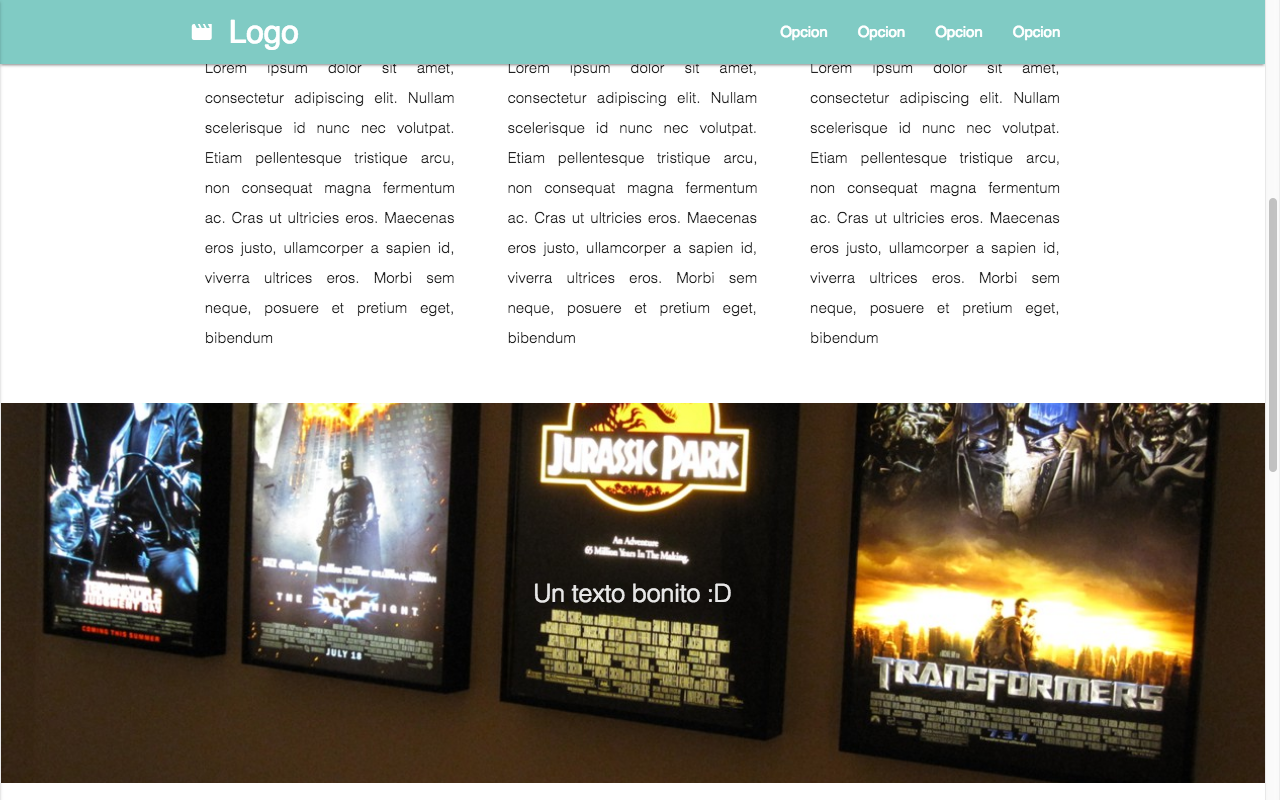
\includegraphics[width=0.80\textwidth]{Examples1.png}
            \caption{Boceto de FrontEnd de la aplicación web}
        \end{figure}



    % ===============================================================
    % =====================    PROBLEMATICA    ======================
    % ===============================================================
    \clearpage
    \section{Problemática}
        
        Buscamos crear un sitema que permita organizar toda la administración de un Cine y todas
        sus subdivisiones de manera consisa, confiable y segura.

        Queremos que dicha aplicación web pueda ser usando con gran facilidad, importando lo menos posible
        el sistema operativo que usen nuestros clientes para usar la aplicación web así como el
        disposivito que utilicen, sea un tablet, un celular o una computadora (de cualquier gana)

        Buscamos que sea de fácil mejoramiento y que podamos actualizar y corregir de la manera más rápida
        cualquier error que tuviera nuestra aplicación web.

        Buscamos que la información que tenga nuestra aplicación web en la base de datos sea de fácil acceso
        para la creación posterior de nuevas interfaces y aplicaciones así como para su mantenimiento
        y escalabilidad.

        Buscamos la mayor seguridad en los datos, de tal manera que sean lo mas confiables posible.

        Buscamos que nuestra aplicación web permita diferentes perfiles de usuarios, para mejorar la confiabilidad
        y seguridad del sistema permitiendo a cierto tipo de usuarios solo hacer ciertas actividades y 
        tener la capacidad de leer / modificar ciertos datos dentro del sistema.



        \begin{figure}[h!]
            \centering
            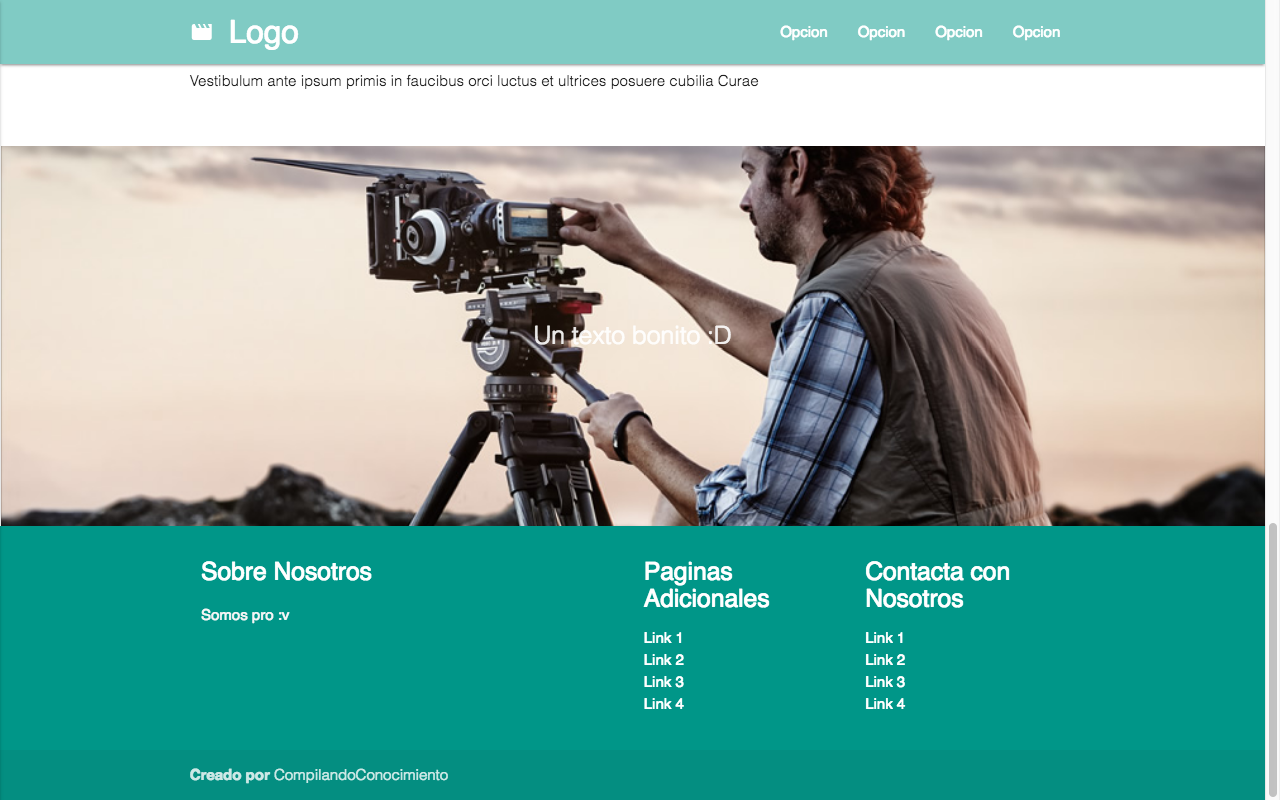
\includegraphics[width=0.80\textwidth]{Examples2.png}
            \caption{Boceto de FrontEnd de la aplicación web}
        \end{figure}




    % ===============================================================
    % =====================     OBJETIVOS      ======================
    % ===============================================================
    \clearpage
    \section{Objetivos}


        % =============================================
        % =====     OBJETIVOS  GENERALES    ===========
        % =============================================
        \subsection{Objetivo General:}

            Desarrollar un sistema que permita gestionar varios de los procesos necesarios en un cine;
            como son la dulcería, la venta de boletos y los roles de empleados.


        % =============================================
        % =====     OBJETIVOS  PARTICULARES    ========
        % =============================================
        \subsection{Objetivos Particulares:}

            \begin{itemize}
                \item A través del desarrollo de un sistema gestionar los horarios de entrada y
                    salida de los empleados en las diferentes áreas del cine.
                
                \item El sistema podrá gestionar los horarios y salas de las diferentes exhibiciones.

                \item El sistema gestionara la venta de boletos para las diferentes exhibiciones,
                    además controlara la disponibilidad de boletos existentes para cada exhibición.

                \item El sistema controlara la dulcería, como la venta de los diferentes artículos,
                    la existencia de estos y los proveedores.

                \item Se permitirá la creación de usuarios para restringir el acceso a la escritura y
                    lectura de los diferentes datos, según el puesto que tenga el usuario en el cine.

            \end{itemize}



    % ===============================================================
    % =====================     REQUERIMIENTOS      =================
    % ===============================================================
    \section{Requerimientos}


        % =============================================
        % =====      REGLAS DE NEGOCIO      ===========
        % =============================================
        \subsection{Reglas de Negocio}

            \begin{tabular}{r ||c |m{7em} | m{15em} |c |c }
               &  ID & Nombre & Descripción & Prioridad & Origen \\ [0.5ex] 
               \hline\hline
              
                & RN1   & Control de Empleados                  &
                Un gerente que lleva el control de los empleado(vendedores de duces boletos y los que limpian)
                & Alta  & Propuestos\\

                & RN2   & Pagos                                 &
                El gerente se encarga de el pago a los proveedores
                & Media  & Propuestos\\

                & RN3   & Control de Salas                      &
                El gerente se encargar de determinar las salas para una pelicula y los horarios
                & Media  & Propuestos\\


                & RN4   & Control de Dulcería                   &
                Se debe de poder seleccionar los dulces y bebidas disponibles por ese día, 
                se venden 5 tipos diferentes de combos, el cliente debe elegir cual de los
                5 desea o puede no comprar ninguno.
                & Media  & Propuestos\\

                & RN4   & Control de Capacidad                   &
                Existen 6 salas, las cuales a su vez tienen 30 butacas, por lo que debe controlarse el numero
                de personas que entran.

                Al tratarse de un cine popular, solo se exhiben peliculas nuevas, y las tarifas de licencia
                para exhibir películas, las cuales pueden ser muy altas, sobre todo para películas importantes
                de estreno (puedes contratar a agentes de cine para ayudar con el proceso de conseguir las
                películas y la aprobación para exhibirlas)
                & Baja  & Propuestos\\

            \end{tabular}


        % =============================================
        % =====     REQUERIMIENTOS BASICOS  ===========
        % =============================================
        \clearpage
        \subsection{Requerimientos Básicos}

            \begin{tabular}{r ||c |m{7em} | m{15em} |c |c }
               &  ID & Nombre & Descripción & Prioridad & Origen \\ [0.5ex] 
               \hline\hline
              
                & RB1   & Seguridad                         &
                Todas las conexiones con la base de datos, así como la confiabilidad de los datos
                tienen que ser altas, para una mayor seguridad.
                & Alta  & Propuestos\\

                & RB2   & Compatibilidad de Navegadores     &
                El sistema tiene que ser accesible desde los navegadores mas usados
                & Baja  & Propuestos\\

                & RB3   & Compatibilidad de Plataformas     &
                El sistema puede ser usado desde diversas plataformas
                & Baja  & Propuestos\\

                & RB4   & Escalabilidad                     &
                La estructura tanto de la aplicación web como de la base de datos a nivel conceptual tiene
                que permitir el mantenimiento y la escalabilidad el proyecto.
                & Media  & Propuestos\\

                & RB4   & Roles                             &
                La aplicación web permite la existencia de distintos tipos de usuarios, con cada tipo
                las acciones disponibles cambian.
                & Media  & Propuestos\\

            \end{tabular}


        % =============================================
        % =====   REQUERIMIENTOS FUNCIONALES    =======
        % =============================================
        \subsection{Requerimientos Funcionales}

            \begin{tabular}{r ||c |c | m{15em} |c }
               &  ID & Nombre & Descripción & Origen \\ [0.5ex] 
               \hline\hline
              
                & RF1 & Gestionar Sala          &
                El Sistema permitirá al usuario gerente establecer los horarios y peliculas para una sala
                & RN2\\
                & RF2 & Gestionar Empleados     & 
                El sistema permitirá establecer que actividad llevará a cabo cada empleado impliendole
                realizar otra que no sea la indicada
                & RN1\\
                & RF3 & Control de Suministros  &
                El sistema podrá llevar stock de todos los productos utilizados en venta o en mantenimiento del cine
                & RN3\\
                & RF4 & Control de Entradas     &
                El sistema deberá indica el estatus de una sala al realizar la venta de un boleto en ella
                & RN6\\
                & RF5 & Gestión de Dulcería     & 
                El sistema permitira manejar las transacciones de venta en el departamento de dulceria
                & RN5\\
            \end{tabular}


        % =============================================
        % ===  REQUERIMIENTOS NO FUNCIONALES    =======
        % =============================================
        \subsection{Requerimientos No Funcionales}
            \begin{tabular}{r ||c |m{8em} | m{18em} |c }
               &   & Nombre & Descripción & Origen \\ [0.5ex] 
               \hline\hline
                & RNF1 & FrameWork &
                Sistema Desarrollado en: JQuery, MaterializeCSS
                & RB3\\

                & RNF2 & Entorno de Trabajo de Aplicaciones &
                PHP, HTML, Javascript, CSS, XAMPP(Apache)  
                & RB2\\

                & RNF3 & Bases de Datos & MySQL Server
                & RB1\\

                & RNF4 & Seguridad & Confidencia e integridad de los datos
                & RB1\\
            \end{tabular}


    % ===============================================================
    % =====================    DIAGRAMA DE CONTEXTO   ===============
    % ===============================================================
    \clearpage
    \section{Diagrama de Contexto}

        \begin{figure}[h]
            \centering
            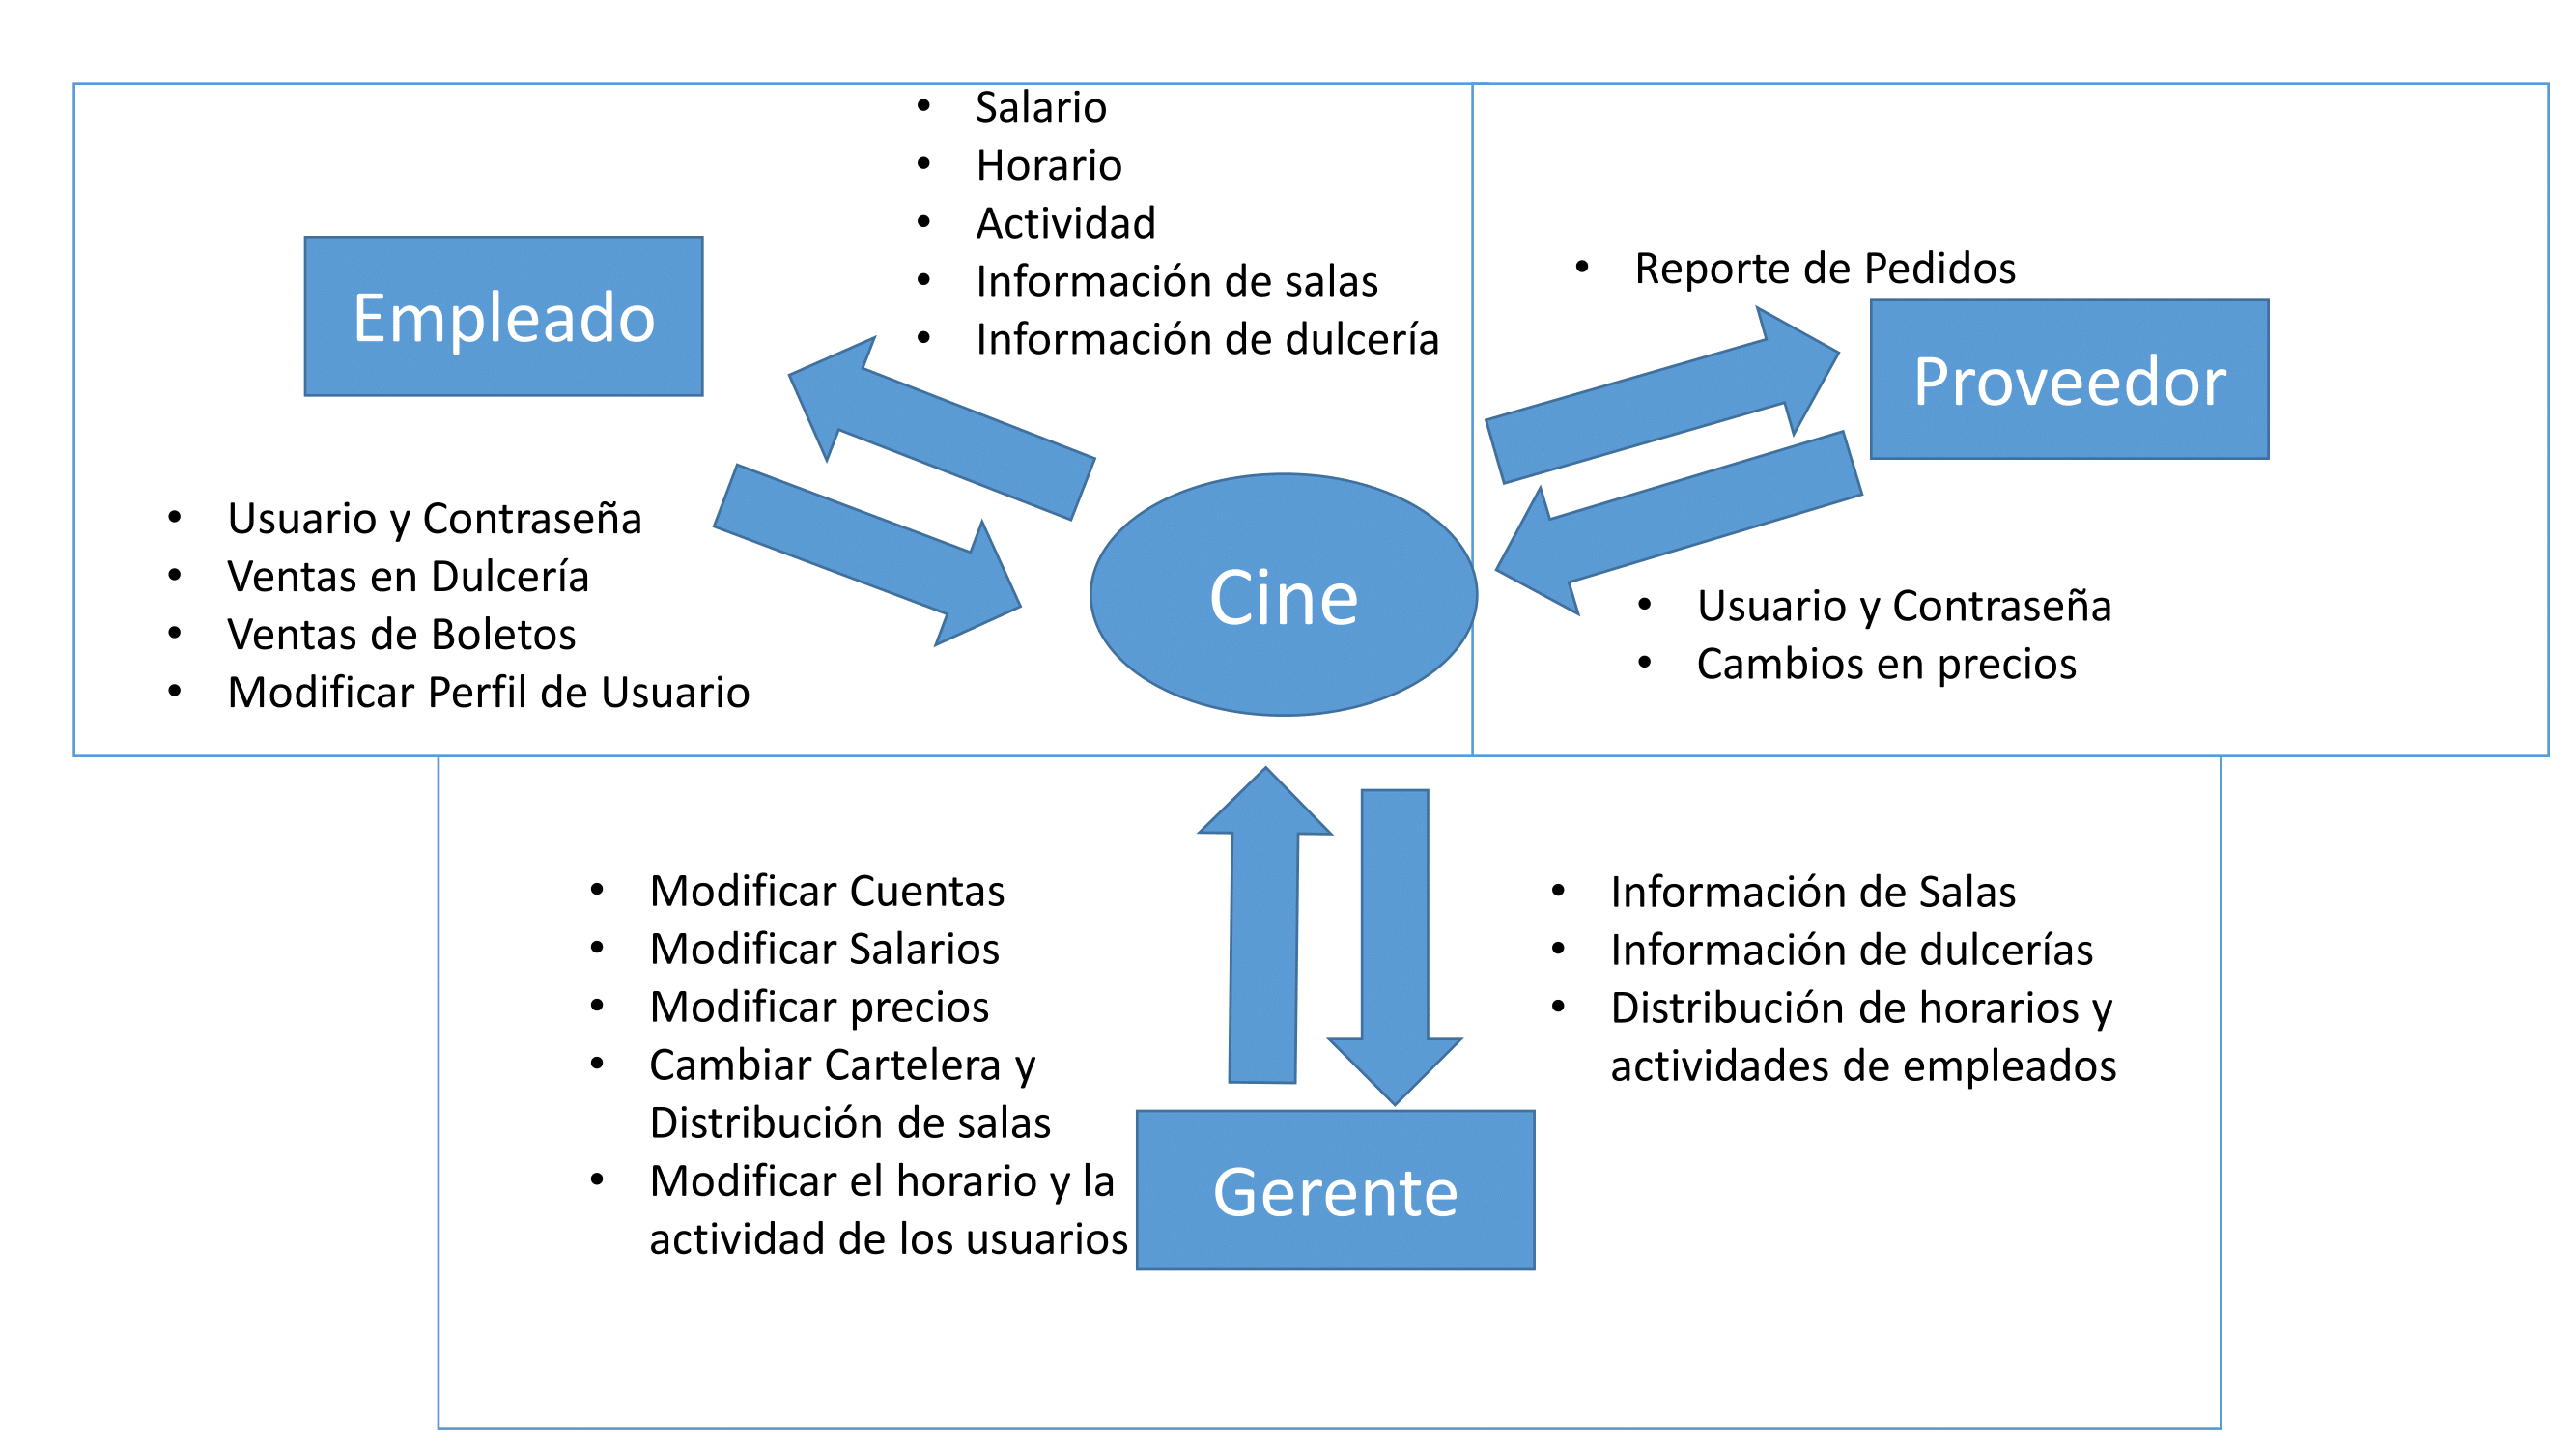
\includegraphics[width=0.85\textwidth]{DiagramaContexto}
        \end{figure}


    % ===============================================================
    % =====================   ANALISIS DE RIEGOS      ===============
    % ===============================================================
    \clearpage
    \section{Análisis de Riesgos}

        % =====================================
        % =====   RIESGOS EN GENERAL    =======
        % =====================================
        \subsection{Riesgos en General}

            \begin{tabular}{r ||  m{12em} | m{12em} | c | c }
               &  Riesgos & Categorias & Probabilidad & Impacto \\ [0.5ex] 
               \hline\hline
              
                & Fecha de Entrega será apretada
                & Riesgo de Calendario  
                & 60\%
                & Marginal
                \\
                \hline

                & Fecha de Capacitación con las Herramientas
                & Riesgo de Apoyo  
                & 50\%
                & Despreciable
                \\
                \hline

                & Personal inexperto en el Sistema
                & Riesgo de Apoyo  
                & 70\%
                & Marginal
                \\
                \hline

                & Mayor número de usuarios que el esperado
                & Riesgo de Apoyo
                & 30\%
                & Crítico
                \\
                \hline

                & Personal renunciando al proyecto
                & Riesgo de Apoyo
                & 40\%
                & Crítico
                \\
                \hline

                & Personal accidentado
                & Riesgo de Apoyo
                & 10\%
                & Marginal
                \\
                \hline

                & Usuario finales ser resisten a la interfaz
                & Riesgo de Rendimiento
                & 20\%
                & Marginal
                \\
                \hline

                & Implementación de algún requisito fallida
                & Riesgo de Rendimiento
                & 70\%
                & Catastrófico
                \\
                \hline

            \end{tabular}

        % =====================================
        % =====   RIESGOS EN GENERAL    =======
        % =====================================
        \clearpage
        \subsection{Hoja de Riesgos}


            Ahora veamos en más detalle como es los riesgos
            que tienen un impacto mayor al 30\%


            \textbf{Riesgo: El personal renuncia del proyecto por
            diferentes causas}

                % ======== DEMOSTRACION ========
                \begin{SmallIndentation}[1em]
                    \textbf{Hoja de Riesgo}:
                    
                    \begin{itemize}
                        \item Probabilidad 40\%
                        \item Impacto Crítico
                        \item
                            \textbf{Refinamiento / Contexto}
                            \begin{itemize}
                                \item 
                                    Los integrantes de quipo pueden
                                    decidir dejar de tomar la materia por falta
                                    de tiempo

                                \item
                                    Pueden tener malas calificaciones y decidir
                                    dejar de trabajar al final del semestre

                                \item
                                    Desacuerdos entre los integrantes del 
                                    equipo que provoquen que alguno abandone
                                    el proyecto 
                            \end{itemize}
                        \item
                            \textbf{Mitigación}
                            \begin{itemize}
                                \item 
                                    Todos los integrantes del equipo deben
                                    estar al pendiente de los últimos avances
                                    del proyecto

                                \item
                                    Todos deben tener copia del proyecto

                                \item
                                    Hacer comprensibles las diferentes
                                    implementaciones del proyecto 
                            \end{itemize}

                        \item
                            \textbf{Plan de Contigencia}

                                Repartir las actividades que realizará en 
                                integrante que ha abandonado entre los 
                                integrantes restantes del equipo


                    \end{itemize}
                
                \end{SmallIndentation}


            \textbf{Riesgo: Durante la implementación alguna parte resulta
            disfuncional}

                % ======== DEMOSTRACION ========
                \begin{SmallIndentation}[1em]
                    \textbf{Hoja de Riesgo}:
                    
                    \begin{itemize}
                        \item Probabilidad 60\%
                        \item Impacto Catastrófico
                        \item
                            \textbf{Refinamiento / Contexto}
                            \begin{itemize}
                                \item 
                                    En ocasiones puede haber errores en la
                                    implementación de la aplicación web

                                \item
                                    Incompatibilidad entre navegadores o entre
                                    sistemas operativos

                                \item
                                    Se ignoro alguno requisito durante la
                                    implementación
                            \end{itemize}
                        \item
                            \textbf{Mitigación}
                            \begin{itemize}
                                \item 
                                    Mantener siempre informados a los integrantes
                                    de los requisitos del proyecto

                                \item
                                    Comunicar entre los integrantes del equipo
                                    la manera en que se implementará el proyecto
                                    para evitar incompatibilidades

                                \item
                                    Realizar un código comentado y facil de 
                                    comprender para facilitar la detección de 
                                    errores
                            \end{itemize}

                        \item
                            \textbf{Plan de Contigencia}

                                Tener un alternativa sencilla aunque pocos 
                                eficiente para la implementación de los 
                                diferentes componentes del proyecto

                    \end{itemize}
                
                \end{SmallIndentation}
                    



% ======================================================================================
% ===============================   SEGUNDA PARTE     ==================================
% ======================================================================================
\chapter{Segunda Parte}
\clearpage

    % ===============================================================
    % =====================     ENTIDAD RELACION   ==================
    % ===============================================================
    \clearpage
    \section{Entidad Relación}


    % ===============================================================
    % ===============      MODELO RELACIONAL       ==================
    % ===============================================================
    \clearpage
    \section{Modelo Relacional}

        % =============================================
        % =====    DIAGRAMAS CON WORKBENCH      =======
        % =============================================
        \subsection{Diagrama Relacional con MySQLWorkBench}

            \begin{figure}[h]
                \centering
                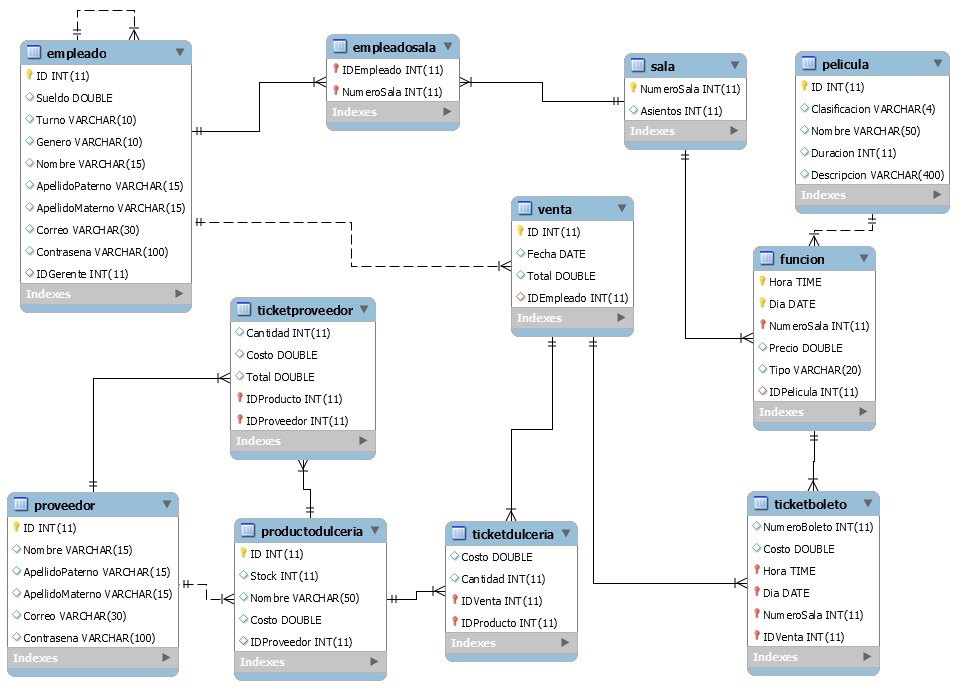
\includegraphics[width=0.95\textwidth]{DataBase/Relations2.png}
            \end{figure}

        % =============================================
        % ========   CODIGO EN SQL     ================
        % =============================================
        \clearpage
        \subsection{Codigo en SQL}

            \lstinputlisting[language=SQL,linerange={1-43}]
            {DataBase/DataBaseTables.sql}
            \clearpage

            \lstinputlisting[language=SQL,linerange={46-91}]
            {DataBase/DataBaseTables.sql}
            \clearpage

            \lstinputlisting[language=SQL,linerange={94-140}]
            {DataBase/DataBaseTables.sql}
            \clearpage

            \lstinputlisting[language=SQL,linerange={143-181}]
            {DataBase/DataBaseTables.sql}



    % ===============================================================
    % ===============      DICCIONARIO DE DATOS      ================
    % ===============================================================
    \clearpage
    \section{Diccionario de Datos}


        \subsection*{Relación: Función}

            Aquella relación que almacena los datos que caracterizan a la presentación
            de una película a una hora determinada, en una sala específica.

            Una película puede presentarse en varias funciones y varias funciones pueden
            presentarse en una sala.

            \vspace{2em}

            \small{
            \begin{tabular}{| c | c | c |}
                \hline
                \textbf{Campo} & \textbf{Tipo de Datos (tamaño)} & \textbf{Constraint} \\[0.5ex] 
                \hline\hline
                
                Hora        & TIME          & PK                        \\
                Dia         & DATE          & PK                        \\
                NumeroSala  & INT(11)       & PK , FK                   \\
                Precio      & REAL          &                           \\
                Tipo        & VARCHAR(20)   &                           \\
                IDPelicula  & INT(11)       & FK                        \\
                \hline
            \end{tabular}
            }


        \subsection*{Relación: Película}

            Relación que guarda los datos sobre una determinada película, como su
            descripción, clasificación y duración, es necesario saber qué película
            se presenta en cada función, recordando que una película puede presentarse
            en varias funciones, pero una función solo puede presentar una película.

            \vspace{2em}

            \small{
            \begin{tabular}{| c | c | c |}
                \hline
                \textbf{Campo} & \textbf{Tipo de Datos (tamaño)} & \textbf{Constraint} \\[0.5ex] 
                \hline\hline
                
                ID              & INT (11)         & PK                        \\
                Clasificacion   & VARCHAR(4)       &                           \\
                Nombre          & VARCHAR(50)      &                           \\
                Duracion        & INT(11)          &                           \\
                Descripcion     & VARCHAR(400)     &                           \\
                \hline
            \end{tabular}
            }



        \clearpage
        \subsection*{Relación: TicketBoleto}

            Relación que permite llevar un control sobre los boletos que tiene
            cada función, guardando también las características de la venta.

            \vspace{2em}

            \small{
            \begin{tabular}{| c | c | c |}
                \hline
                \textbf{Campo} & \textbf{Tipo de Datos (tamaño)} & \textbf{Constraint} \\[0.5ex] 
                \hline\hline
                
                NombreBoletos   & INT(11)    &                           \\
                Costos          & REAL       &                           \\
                Hora            & TIME       & PK , FK                   \\
                Dia             & DATE       & PK , FK                   \\
                NumeroSala      & INT(11)    & PK , FK                   \\
                IDVenta         & INT(11)    & PK , FK                   \\
                \hline
            \end{tabular}
            }


        \subsection*{Relación: TicketDulceria}

            Aquella relación que permite tener un control sobre la comida/dulces vendidos.

            \vspace{2em}

            \small{
            \begin{tabular}{| c | c | c |}
                \hline
                \textbf{Campo} & \textbf{Tipo de Datos (tamaño)} & \textbf{Constraint} \\[0.5ex] 
                \hline\hline
                
                Costos          & REAL       &                           \\
                Cantidad        & INT(11)    &                           \\
                IPProducto      & INT(11)    & PK , FK                   \\
                IDVenta         & INT(11)    & PK , FK                   \\
                \hline
            \end{tabular}
            }




        \subsection*{Relación: ProductoDulceria}

            Relación encargada de almacenar los productos de la dulcería, tales como dulces,
            palomitas y refrescos. Se guardan también sus costos y el proveedor que los provee.

            \vspace{2em}

            \small{
            \begin{tabular}{| c | c | c |}
                \hline
                \textbf{Campo} & \textbf{Tipo de Datos (tamaño)} & \textbf{Constraint} \\[0.5ex] 
                \hline\hline
                
                IPProducto      & INT(11)       & PK                    \\
                Stock           & INT(11)       &                       \\
                Nombre          & VARCHAR(50)   &                       \\
                Costo           & REAL          &                       \\
                IDProveedor     & INT(11)       & FK                    \\
                \hline
            \end{tabular}
            }

        \clearpage
        \subsection*{Relación: TicketProoveedor}

            Relación destinada a relacionar los proveedores con los productos de dulcería,
            almacenando la cantidad, el total y la fecha en la que se proporcionaron los dulces,
            por parte del proveedor.

            \vspace{2em}

            \small{
            \begin{tabular}{| c | c | c |}
                \hline
                \textbf{Campo} & \textbf{Tipo de Datos (tamaño)} & \textbf{Constraint} \\[0.5ex] 
                \hline\hline
                
                Fecha       & DATE          &                       \\
                Total       & REAL          &                       \\
                Cantidad    & INT(11)       &                       \\
                IDProducto  & INT(11)       & PK , FK               \\
                IDProveedor & INT(11)       & PK , FK               \\
                \hline
            \end{tabular}
            }

        \subsection*{Relación: Proveedor}

            Aquella relación destinada a almacenar la información del proveedor como
            lo es su nombre y correo (el correo será único, y tendrá su contraseña).

            \vspace{2em}

            \small{
            \begin{tabular}{| c | c | c |}
                \hline
                \textbf{Campo} & \textbf{Tipo de Datos (tamaño)} & \textbf{Constraint} \\[0.5ex] 
                \hline\hline
                
                IDProveedor & INT(11)       & PK                    \\
                Nombre      & VARCHAR(15)   &                       \\
                Apellido1   & VARCHAR(15)   &                       \\
                Apellido2   & VARCHAR(15)   &                       \\
                Correo      & VARCHAR(30)   &                       \\
                Contrasena  & VARCHAR(100)  &                       \\
                \hline
            \end{tabular}
            }


        \subsection*{Relación: EmpleadoSala}

            Relación que asocia al empleado y sala. Viene dada de una cardinalidad
            muchos a muchos, y sirve para almacenar los empleados que revisan una sala,
            y las salas que son revisadas por un empleado.

            \vspace{2em}

            \small{
            \begin{tabular}{| c | c | c |}
                \hline
                \textbf{Campo} & \textbf{Tipo de Datos (tamaño)} & \textbf{Constraint} \\[0.5ex] 
                \hline\hline
                
                ID          & INT(11)       & PK , FK               \\
                NumSala     & INT(11)       & PK, FK                \\
                \hline
            \end{tabular}
            }


        \clearpage
        \subsection*{Relación: Empleado}

            Relación que guarda la información del usuario o cliente, almacenando ambos
            con una relación unitaria para saber que gerente dirige a los usuarios.
            Los usuarios y gerentes de distinguen entre sí por el campo rol.
            Un gerente puede dirigir a varios empleados, pero un empleado solo tiene un gerente.

            \vspace{2em}

            \small{
            \begin{tabular}{| c | c | c |}
                \hline
                \textbf{Campo} & \textbf{Tipo de Datos (tamaño)} & \textbf{Constraint} \\[0.5ex] 
                \hline\hline
                
                ID          & INT(11)       & PK                    \\
                Nombre      & VARCHAR(15)   &                       \\
                Apellido1   & VARCHAR(15)   &                       \\
                Apellido2   & VARCHAR(15)   &                       \\
                Correo      & VARCHAR(30)   &                       \\
                Contrasena  & VARCHAR(100)  &                       \\
                Sueldo      & REAL          &                       \\
                Turno       & VARCHAR(10)   &                       \\
                Rol         & VARCHAR(15)   &                       \\
                Genero      & VARCHAR(10)   &                       \\
                IDGerente   & INT(11)       & FK                    \\
                NumEmpleados& INT(11)       &                       \\
                ID\_Ger     & INT(11)       & FK (Llave recursiva)  \\
                \hline
            \end{tabular}
            }

        \subsection*{Relación: Sala}

            Aquella relación que almacena las salas y el número de asientos disponible
            en cada una.

            \vspace{2em}

            \small{
            \begin{tabular}{| c | c | c |}
                \hline
                \textbf{Campo} & \textbf{Tipo de Datos (tamaño)} & \textbf{Constraint} \\[0.5ex] 
                \hline\hline
                
                ID          & INT(11)       & PK                    \\
                Asientos    & INT(11)       &                       \\
                \hline
            \end{tabular}
            }










    % ===============================================================
    % =======================    CASOS DE USOS       ================
    % ===============================================================
    \clearpage
    \section{Diagrama de Casos de Uso}

        \begin{figure}[h]
            \centering
            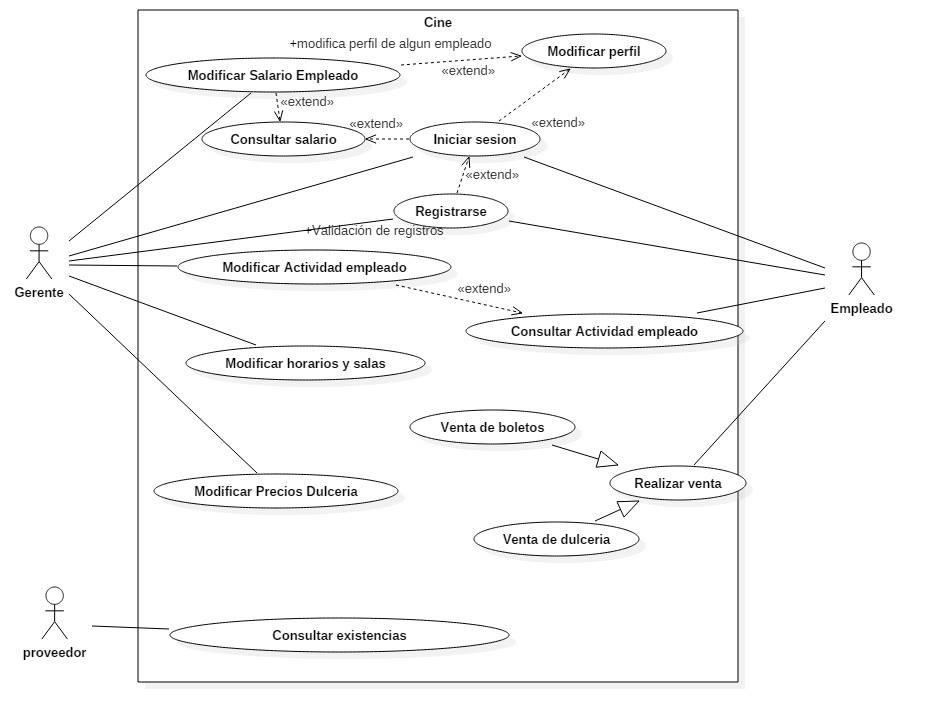
\includegraphics[width=0.95\textwidth]{DiagramasDeCasosDeUso}
        \end{figure}

    % ===============================================================
    % ==================  DIAGRAMA SECUENCIAL        ================
    % ===============================================================
    \clearpage
    \section{Diagrama Secuencial}


        \begin{figure}[ht]
            \centering
            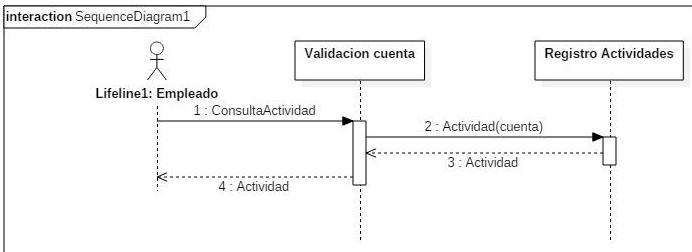
\includegraphics[width=0.85\textwidth]{DiagramaSecuencial1}
            \caption{Consultar Actividad}
        \end{figure}


        \begin{figure}[ht]
            \centering
            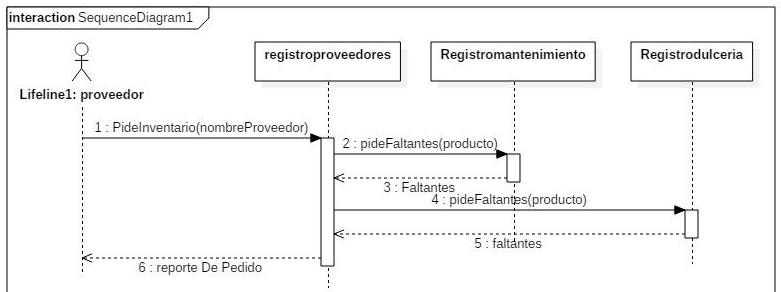
\includegraphics[width=0.65\textwidth]{DiagramaSecuencial2}
            \caption{Consultar Existencias}
        \end{figure}

        \begin{figure}[ht]
            \centering
            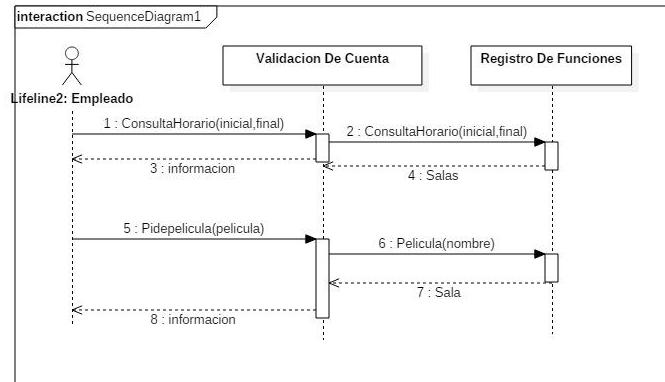
\includegraphics[width=0.85\textwidth]{DiagramaSecuencial3}
            \caption{Consultar Horarios y Salas}
        \end{figure}


        \begin{figure}[ht]
            \centering
            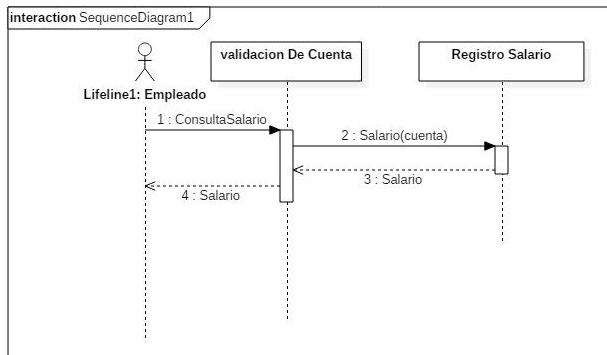
\includegraphics[width=0.65\textwidth]{DiagramaSecuencial4}
            \caption{Consultar Salarios}
        \end{figure}


        \begin{figure}[ht]
            \centering
            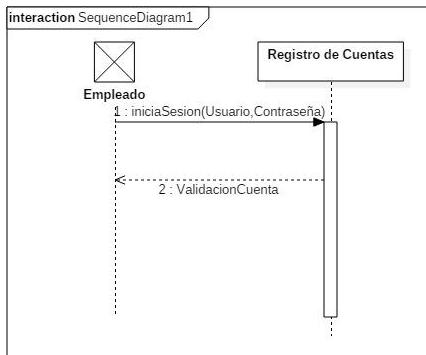
\includegraphics[width=0.65\textwidth]{DiagramaSecuencial5}
            \caption{Iniciar Sesión}
        \end{figure}

        \begin{figure}[ht]
            \centering
            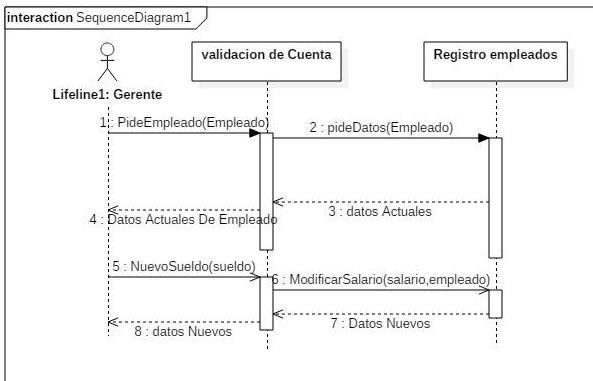
\includegraphics[width=0.85\textwidth]{DiagramaSecuencial6}
            \caption{Modificar Actividad Empleado}
        \end{figure}


        \begin{figure}[ht]
            \centering
            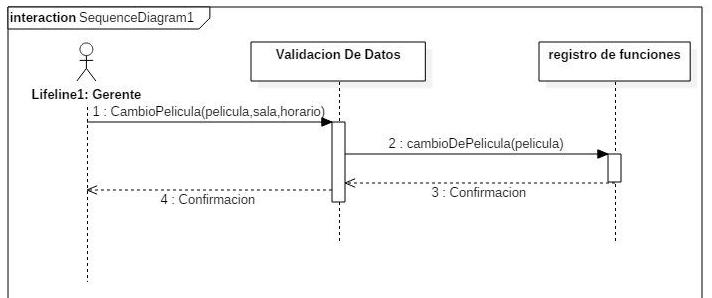
\includegraphics[width=0.65\textwidth]{DiagramaSecuencial7}
            \caption{Modificar Horarios Salas}
        \end{figure}
        
        \begin{figure}[ht]
            \centering
            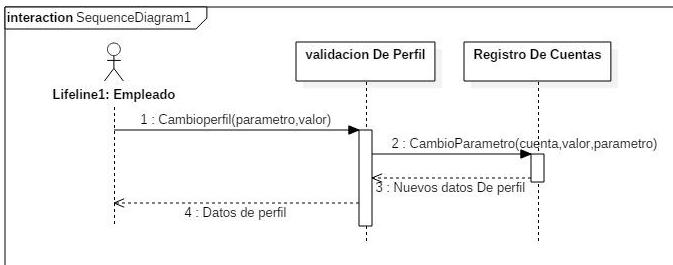
\includegraphics[width=0.85\textwidth]{DiagramaSecuencial8}
            \caption{Modificar Perfil}
        \end{figure}


        \begin{figure}[ht]
            \centering
            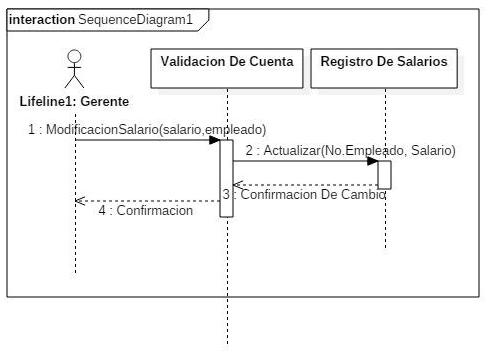
\includegraphics[width=0.65\textwidth]{DiagramaSecuencial9}
            \caption{Modificar Precios Dulcería}
        \end{figure}

        \begin{figure}[ht]
            \centering
            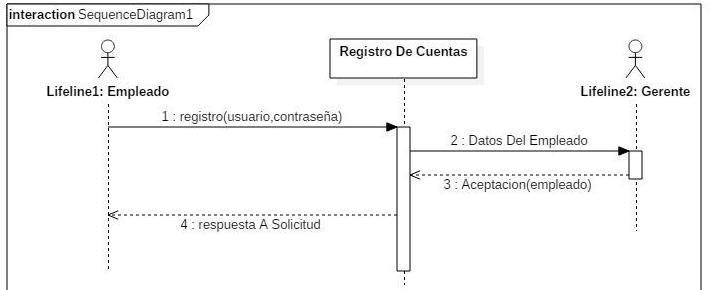
\includegraphics[width=0.85\textwidth]{DiagramaSecuencial10}
            \caption{Modificar Salario}
        \end{figure}


        \begin{figure}[ht]
            \centering
            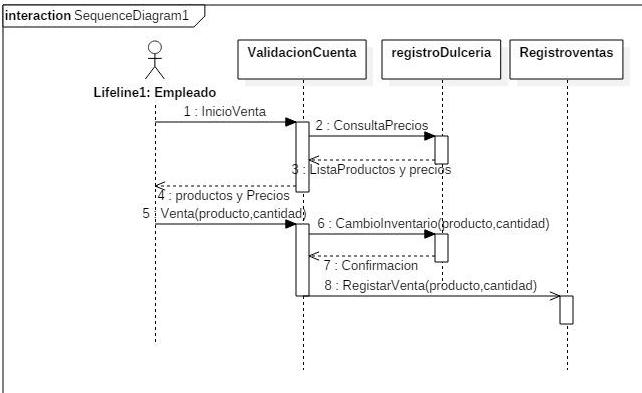
\includegraphics[width=0.65\textwidth]{DiagramaSecuencial11}
            \caption{Registrarse}
        \end{figure}


        \begin{figure}[ht]
            \centering
            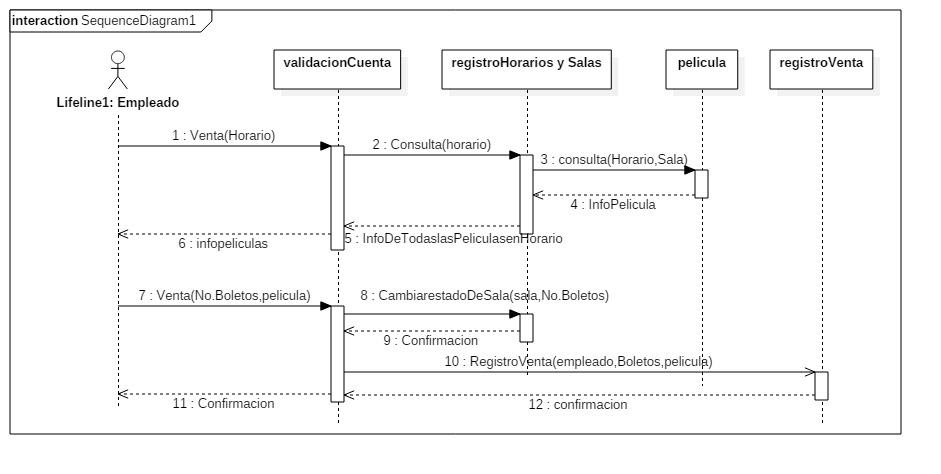
\includegraphics[width=0.65\textwidth]{DiagramaSecuencial12}
            \caption{Venta Boletos}
        \end{figure}


    % ===============================================================
    % ==================  AVANCES DE LA INTERFAZ      ===============
    % ===============================================================
    \clearpage
    \section{Avance de la Interfaz}

        \begin{figure}[ht]
            \centering
            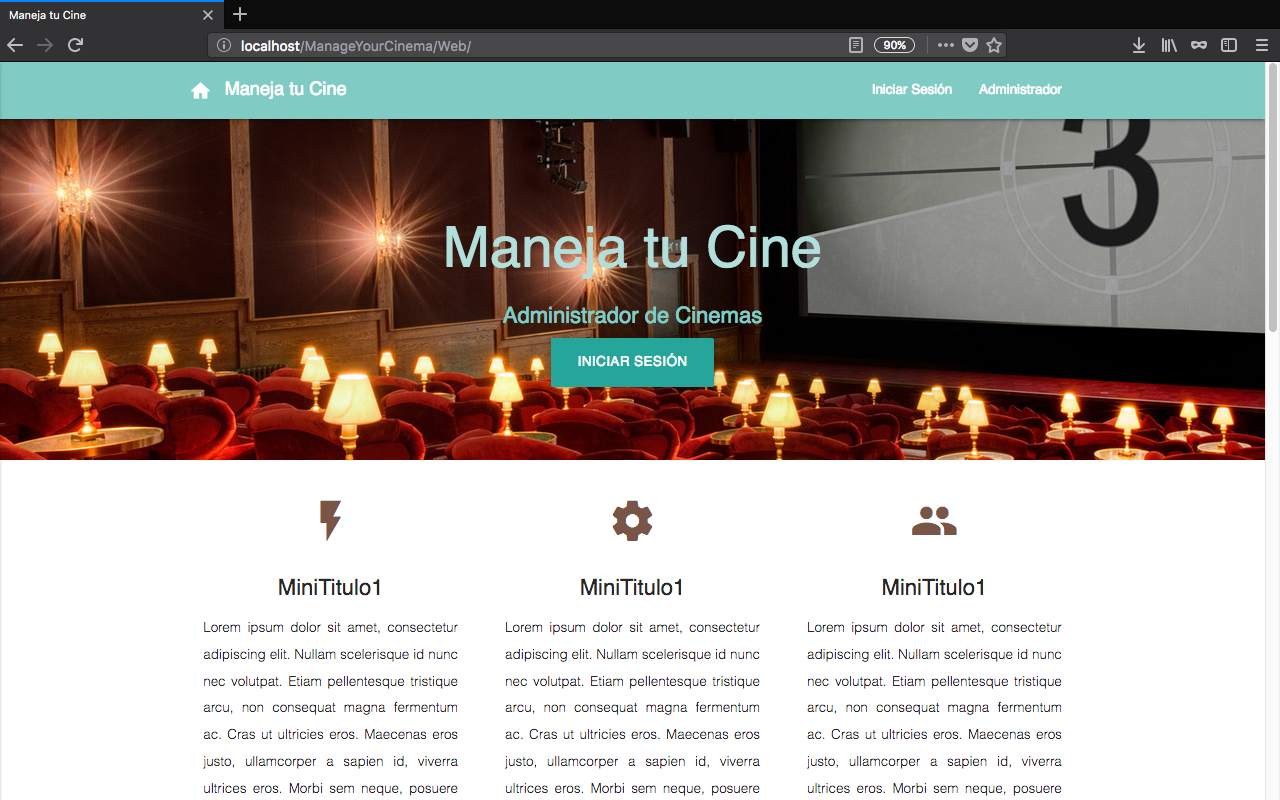
\includegraphics[width=0.65\textwidth]{EjemploInterfazSegundaParte1}
            \caption{Página Principal}
        \end{figure}


        \begin{figure}[ht]
            \centering
            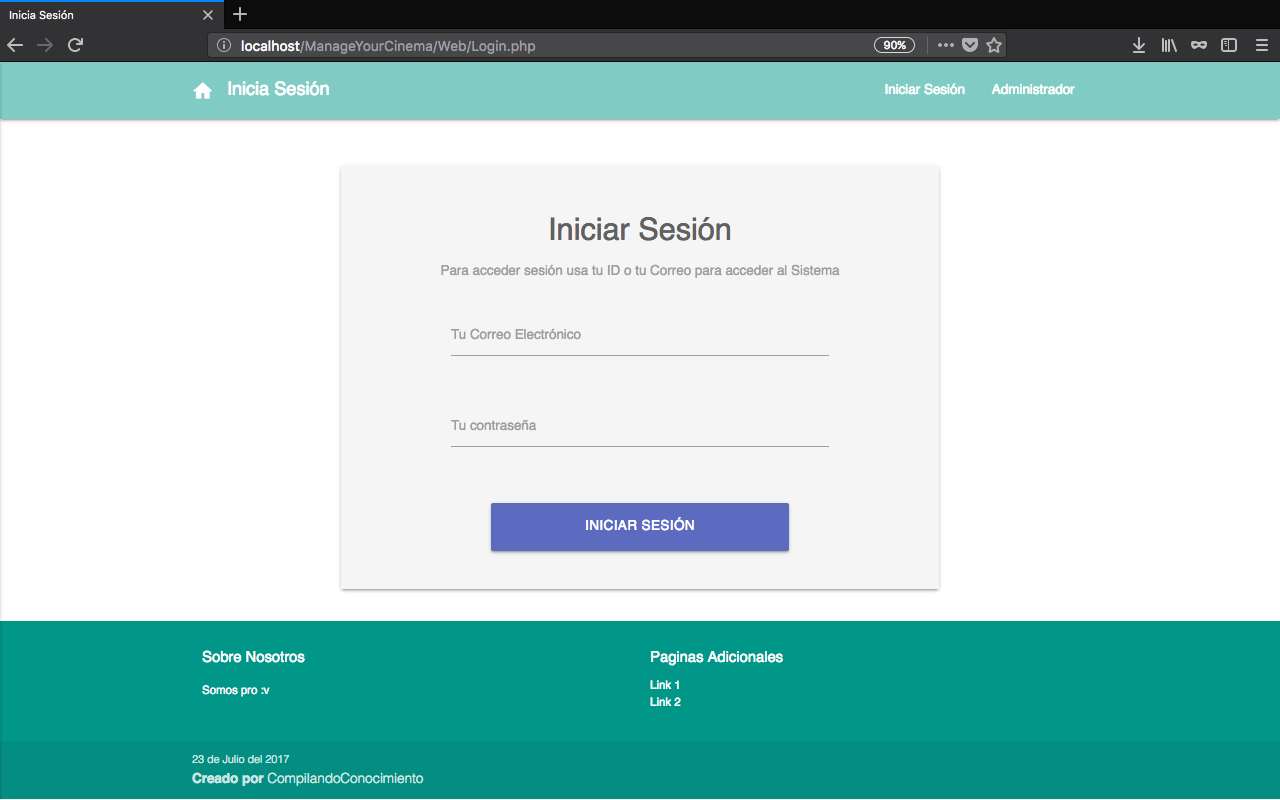
\includegraphics[width=0.65\textwidth]{EjemploInterfazSegundaParte2}
            \caption{Menú de Inicio}
        \end{figure}

        \begin{figure}[ht]
            \centering
            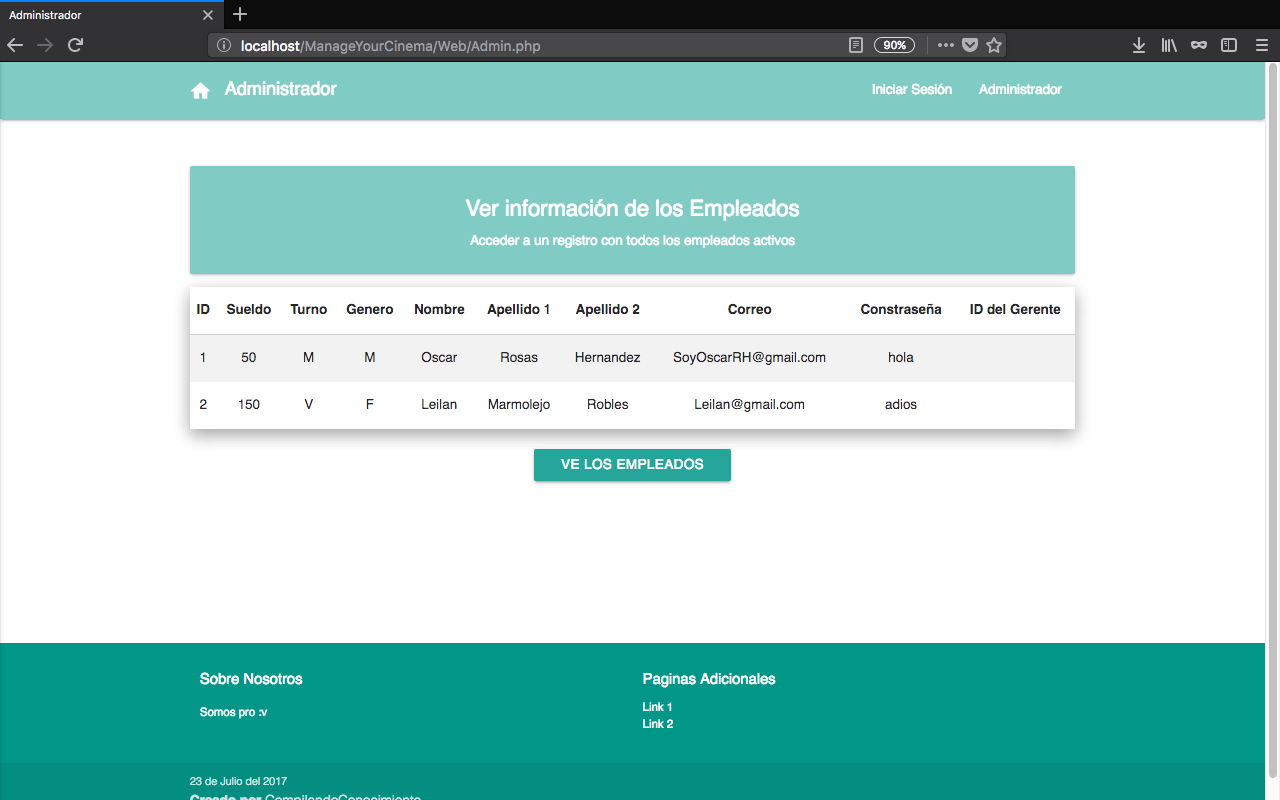
\includegraphics[width=0.65\textwidth]{EjemploInterfazSegundaParte3}
            \caption{Tabla que muestra los Datos}
        \end{figure}

        \begin{figure}[ht]
            \centering
            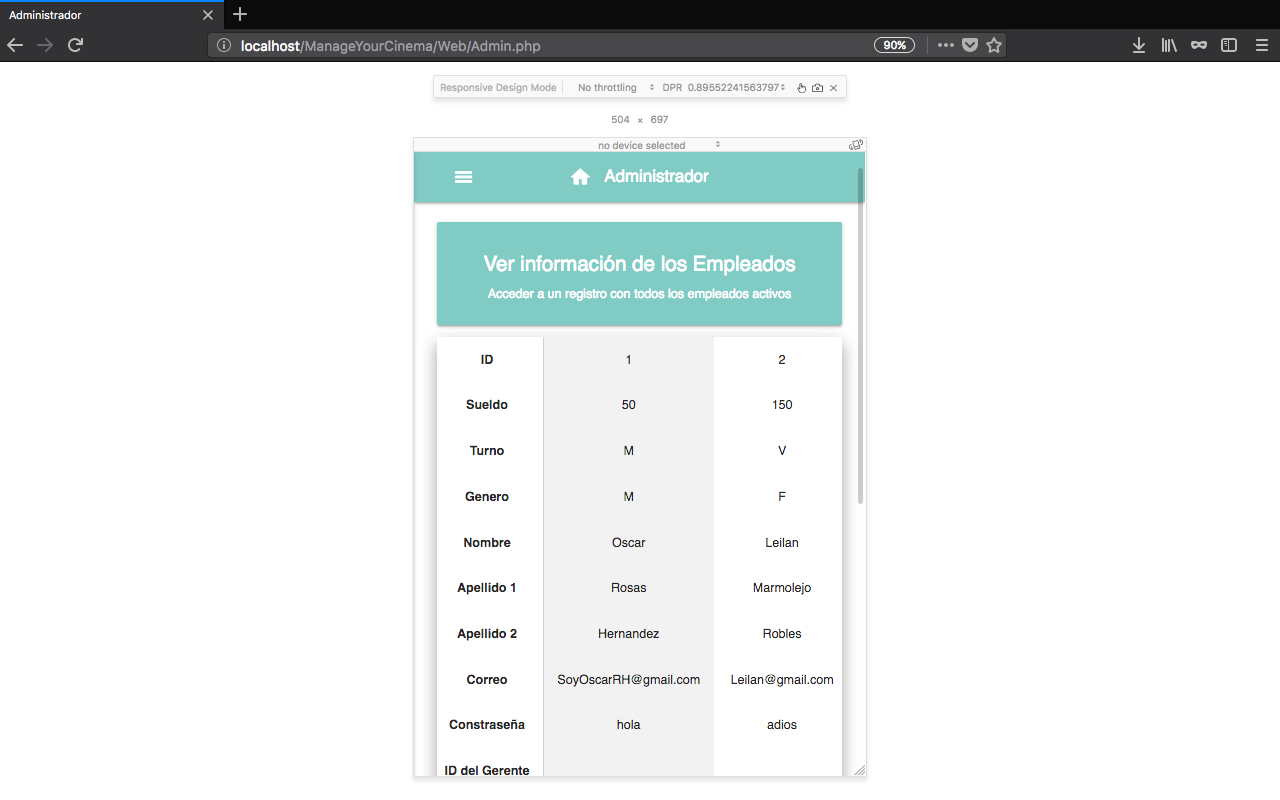
\includegraphics[width=0.65\textwidth]{EjemploInterfazSegundaParte4}
            \caption{Empezamos a hacerlo Responsive para pantallas pequeñas (modificación del menú y creamos menú hamburguesa)}
        \end{figure}

        \begin{figure}[ht]
            \centering
            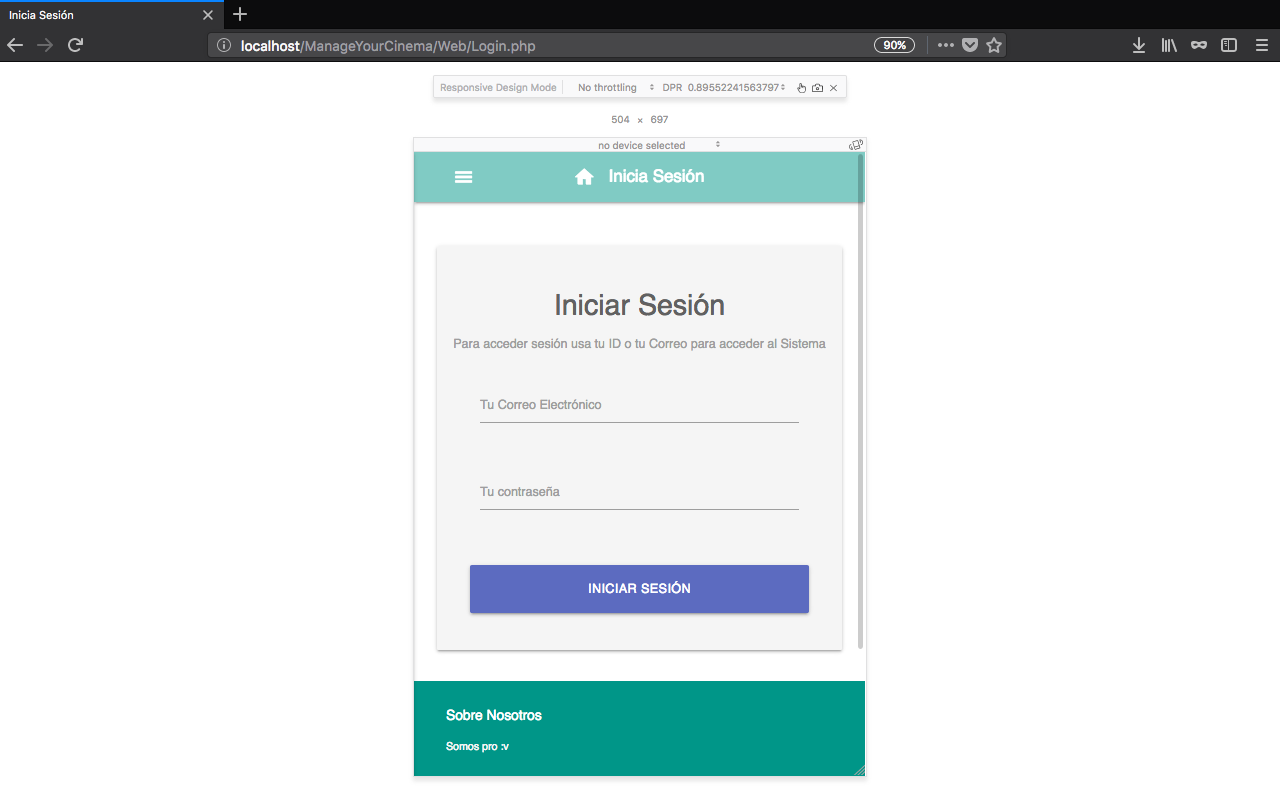
\includegraphics[width=0.65\textwidth]{EjemploInterfazSegundaParte5}
            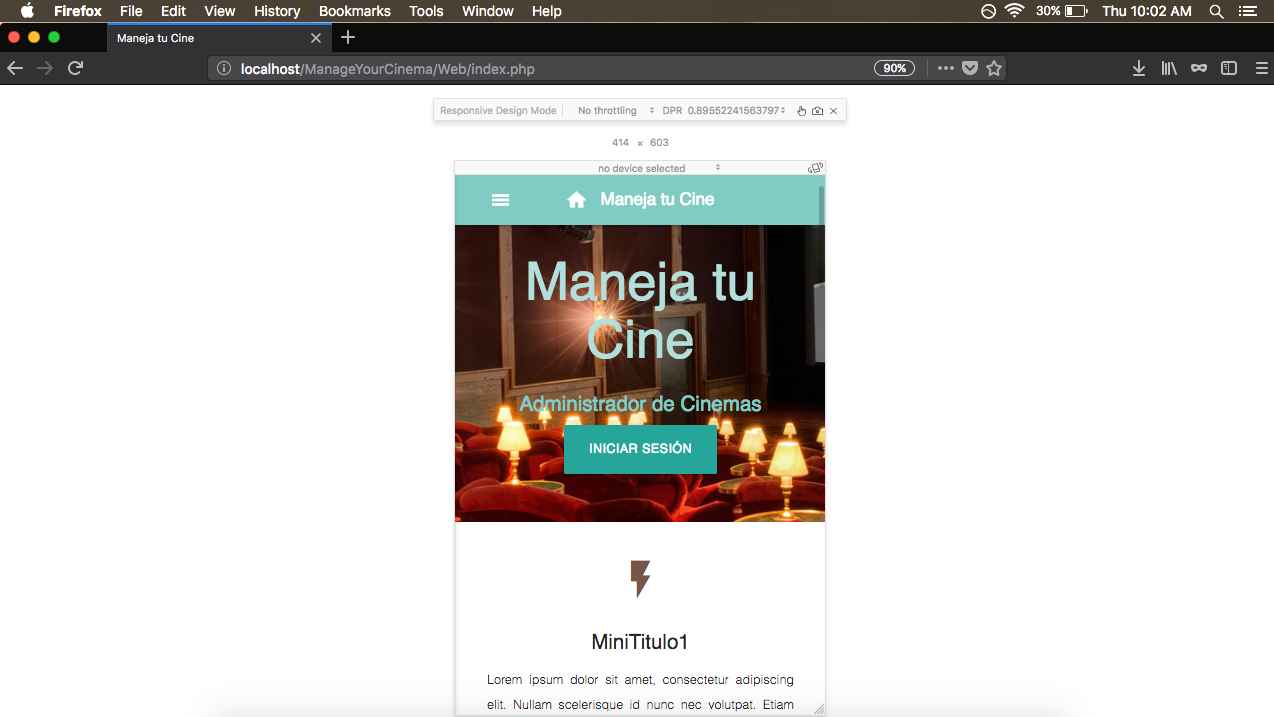
\includegraphics[width=0.65\textwidth]{EjemploInterfazSegundaParte7}
            \caption{Empezamos a hacerlo Responsive para pantallas pequeñas (modificación del menú y creamos menú hamburguesa)}
        \end{figure}


        \begin{figure}[ht]
            \centering
            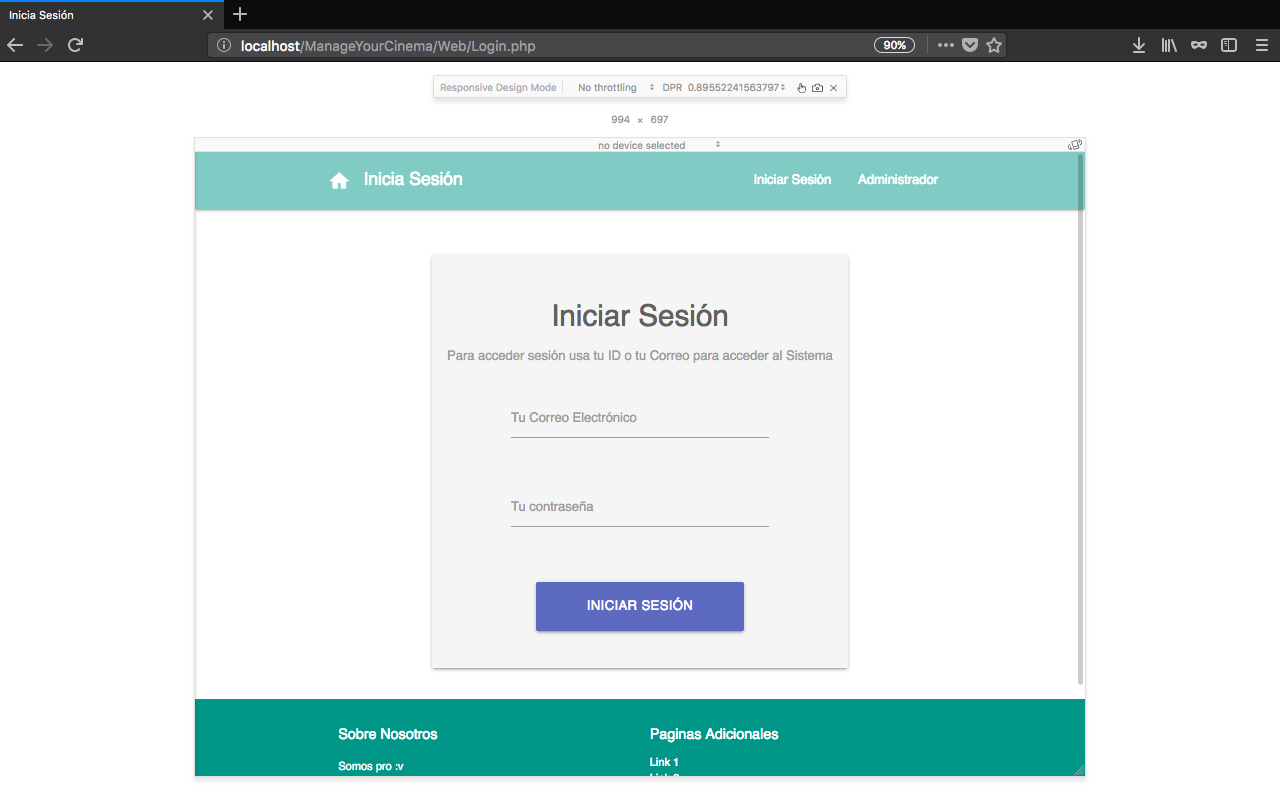
\includegraphics[width=0.65\textwidth]{EjemploInterfazSegundaParte6}
            \caption{Empezamos a hacerlo Responsive para pantallas medianas}
        \end{figure}



    












\end{document}
